
\chapter{Screening and discovery of metal compound active sites for strong and selective adsorption of N$_2$ in air}

\section*{Introduction}
\label{introduction}
The production of ammonia (NH$_3$) from atmospheric nitrogen on an industrial scale is accomplished through the Haber-Bosch process \cite{Schloegl_2003}, which has been called the most important invention of the 20$^{\mathrm{th}}$ century \cite{Smil_1999}. As the main ingredient in nitrogen-based fertilizers, ammonia has directly helped increase food production, enabling the global population to nearly quadruple in the early 20$^{\mathrm{th}}$ century \cite{Smil_1999}. Despite its impressive positive impact on fertilizer production, the Haber-Bosch process is energy and emissions intensive \cite{norskov_2016, SCHIFFER_2017, Comer2019ProspectsFertilizers}. Emitting 340 million tonnes of CO$_2$ equivalent per year and consuming 2.5 exajoule energy per year, ammonia synthesis has become one of the most carbon and energy intensive processes in the chemical industry \cite{Liu2022ProspectsFixation, Comer_sustainable, Comer2019ProspectsFertilizers,Suryanto2021NitrogenShuttle}. The cost of energy consumption is mainly controlled by the production of molecular hydrogen and nitrogen feedstocks \cite{Comer2019ProspectsFertilizers, Etienne2016PriceMarkets, Huang2007ImpactSupply}. Molecular hydrogen is produced via methane steam reforming that contributes to 340 million tonnes of CO$_2$ equivalent per year \cite{Abbas_2010}. Molecular nitrogen is obtained from cryogenic distillation, which requires 6.9 kJ per mol N$_2$ \cite{Taniguchi2015EnergyAnalysis}. Furthermore, the highly centralized ammonia production process leads to high distribution costs and inequitable distribution of fertilizers throughout the world, especially in developing areas \cite{ COMER_2019,Medford_2017, Gilbert_2012}. These downsides of the Haber-Bosch process push the need to develop alternative catalytic systems that enable sustainable and economical fixed nitrogen production in a distributed manner. 

Photo(electro)catalytic nitrogen fixation has the potential to produce ammonia under ambient conditions \cite{Chen2017ElectrocatalyticElectrocatalyst, Chen2018BeyondTransformations, Skulason_2012, Iriawan_2021, Comer2018TheTitania, Comer2018AnalysisTiO2110,Montoya2015TheRelations,Medford2017Photon-DrivenOutlook, Vojvodic2014ExploringProcess}. Photocatalytic ammonia synthesis has shown particular promise as a low capital and highly distributed alternative \cite{Comer2019ProspectsFertilizers}, but current efficiencies indicate that significant additional research is required. Current progress on photocatalytic nitrogen fixation has provided valuable insights regarding the mechanism at a molecular scale. 

One of the first computational studies of photocatalytic nitrogen fixation was performed by Comer and Medford \cite{Comer_sustainable}. This theoretical study explored both dissociative and associative nitrogen reduction on rutile (110) TiO$_2$ active sites, including pristine, oxygen vacancies and iron substitution sites using density functional theory (DFT). However, the results indicated a thermodynamic barrier that is higher than the conduction band edge of rutile TiO$_2$. The interaction between surface hydroxyl groups and nitrogen radicals was also explored in a theoretical study by Xie et al \cite{Xie_2019}. It was suggested that the hydroxyl groups produced by surface hydroxylation of water \cite{edwards1992opinion, Schaub_2001, Henderson1996, Krischok_2001, Ketteler_2007} on titania surfaces could drive the nitrogen reduction process, although no direct experimental evidence was provided. An alternative hypothesis proposed by Comer et al. in a study based on ambient pressure X-ray photoelectron spectroscopy and DFT calculations \cite{Comer2018}, where a carbon substitution site on rutile TiO$_2$ and demonstrated a thermodynamically feasible carbon-assisted nitrogen reduction reaction (NRR) pathway. %This study provides a possible explanation for the photocatalytic nitrogen fixation on titania. 
Building on this observation, Huang et al. \cite{Huang2023FormationIllumination} used electron paramagnetic resonance, infrared spectroscopy, and DFT to show that radical species derived from methanol also interact with nitrogen, providing a more detailed perspective on carbon-assisted nitrogen dissociation.

Despite current progress in probing the mechanistic pathway of photo(electro)catalytic NRR, these mechanisms typically assume a pure nitrogen feedstock, and issues of competitive adsorption in the presence of molecular oxygen have not been explored. To achieve the ultimate goal of NRR under ambient conditions, it will be critical to reduce the need for air separation \cite{Comer2019ProspectsFertilizers}. As mentioned above, the cost of high-purity nitrogen from cryogenic distillation in the Haber-Bosch process accounts for approximately 25\% of the total capital cost of the entire plant \cite{Bartels2008AEconomy}. In the Haber-Bosch process, high purity nitrogen is required to preserve the catalyst and prevent ammonia oxidation \cite{smith_2020}. Furthermore, industrial catalysts used in the process can be poisoned by oxygen or hydroxyl groups below industrial conditions (700 K, 100 bar) \cite{Appl2011AmmoniaProcesses, Rohr2019ACatalysts}. Catalyst poisoning severely hinders the rate of production, which is even more pronounced when water vapor is present \cite{Appl2011AmmoniaProcesses}. Similar phenomena were observed in photocatalytic and electrocatalytic nitrogen fixation experiments. The photocatalytic activity of rutile TiO$_2$ in air has been reported to be reduced by 65\% compared to a high-purity nitrogen environment \cite{Hirakawa_2017}. Under ambient conditions, oxygen can react with photogenerated electrons and holes and turn into reactive oxygen species, decreasing the conversion efficiency \cite{Ye2017Ni2PLight, Huang2020TowardLigands, Comer2018}. Remarkably, a recent study from the electrocatalysis community showed that the Faradaic efficiency and stability of a lithium-mediated NRR can actually be improved by adding small amounts of oxygen, which limits excessive lithium reduction by decreasing the lithium diffusion rate \cite{Li2021EnhancementOxygen}. This is a promising result, but the small amounts of oxygen that enhance the NRR will likely be hard to control and will require further experiments and scale-up studies to assess feasibility. If a nitrogen fixation process is not resistant to contamination from oxygen and other common components under ambient conditions, investment in air separation will be unavoidable and will likely become the dominant capital cost \cite{Comer2019ProspectsFertilizers}. Hence, discovering photocatalysts that are directly compatible with air or low-purity nitrogen is an important step towards enabling the photocatalytic NRR process under ambient conditions \cite{Liu2022ProspectsFixation, Comer2019ProspectsFertilizers}. Furthermore, finding materials that can selectively adsorb N$_2$ over O$_2$ presents a fundamental chemistry challenge, given the relatively high reactivity of O$_2$ compared to N$_2$. These materials may prove interesting as case studies in fundamental chemistry or find applications in other fields such as air separations.


In this work, we propose that the selectivity of adsorbing nitrogen over oxygen is an interesting descriptor of the performance for photocatalytic ammonia synthesis under ambient conditions. Adsorption of N$_2$ is a necessary condition for any N$_2$ conversion process, regardless of the mechanism, so selective adsorption of N$_2$ is a necessary (but not sufficient) condition for aerobic photocatalytic synthesis of ammonia. Employing DFT enables surface adsorption energy calculations, which can be used to predict adsorption selectivity. We quantify the selectivity by comparing the nitrogen and oxygen adsorption free energy on the active site. The inert nature of nitrogen means that many surfaces will not bind it strongly, and if a surface can stably adsorb a nitrogen molecule, it is likely that it can adsorb oxygen even more strongly. Furthermore, this descriptor also provides an implicit approximation of the (meta)stability of a given active site, since extremely unstable active sites are likely to react more strongly with oxygen than nitrogen, particularly for oxides. Therefore, the descriptor will identify metastable active sites with an abnormally strong reactivity toward N$_2$, which we hypothesize will correlate with low barriers for conversion of N$_2$ to ammonia.

Naturally, a thorough description of the photocatalytic performance of a material would require detailed analyses of surface stability, high coverage thermodynamics and reaction barriers, and microkinetic modeling \cite{Motagamwala2021MicrokineticDesign, Peterson_2010}. However, these analyses require a significant amount of resources, which makes them impractical to scale to large search spaces of materials \cite{Wander2022Catlas:Conversion}. Thus, it is often most efficient to utilize relatively simple binding energy descriptors to narrow down the catalyst search space and follow up with more detailed studies of the most promising materials and surfaces. Here, our goal is to expand the breadth of materials studied for photocatalytic nitrogen fixation, and thus we adopt a screening strategy that first uses relatively crude DFT calculations to eliminate surfaces that are not active and selective toward N$_2$ adsorption, and refine the quality of the calculations to obtain a detailed description of the most interesting materials.


In this study, we started with 516 bulk structures of metal oxides, oxyborides, and oxyphosphides from the Materials Project \cite{Jain2013} as candidate photocatalysts. Then, low Miller index (all permutations with a max index of 1) surfaces were generated from each bulk structure. Adsorbate-slab configurations were generated for every active site on a surface. To screen these candidate active sites, we used a two-stage screening strategy. In the first round of low-fidelity screening, we calculate nitrogen and oxygen adsorption energies while holding slab atoms in fixed positions. We then used the binding energy descriptors from low-fidelity calculations to guide the selection of calculations that allowed for surface relaxation and reconstruction. We refer to these subsequent calculations as the "second round screening" throughout this paper. Allowing surface relaxations on metal compounds led to substantial surface reconstructions and significantly weaker N$_2$ adsorption energies in most cases, suggesting that the approach of using a fixed slab is more likely to produce false positives than false negatives, and indicating the importance of considering relaxations in future screening studies. Strong and selective \ce{N2} adsorption was observed in three active sites even after the second round of screening. 

Remarkably, two of the three identified sites occur on meta-stablepolymorphs (space group P3$_1$21 and C2/m) of TiO$_2$, which is one of the most commonly reported catalysts for photocatalytic ammonia synthesis. The other site is on VBO$_4$ (space group P2$_{1/c}$), a material that has not yet been tested for photocatalytic ammonia synthesis. In our detailed investigation, we focused on the (001) surface of a meta-stable trigonal TiO$_2$ P3$_1$21 polymorph \cite{tio2_152}, which demonstrated the highest selectivity for N$_2$ among the TiO$_2$ sites, and the (100) surface of VBO$_4$. 

Using both BEEF-vdW and HSE06 functionals, we performed an extensive thermodynamic analysis of the NRR pathway on these two active sites. The results confirmed that these surfaces show strong and selective reactivity toward N$_2$ and have thermodynamic barriers similar to the (110) rutile TiO$_2$ surface, indicating that meta-stable polymorphs of TiO$_2$ or other oxides may play a role in photocatalytic ammonia synthesis, and that VBO$_4$ may be a promising material for further experimental investigations.


\section*{Methods}
\subsection{DFT calculations}
\label{sec:DFT}
In this work, we used both generalized gradient approximation (GGA) and hybrid level calculations to simulate the electronic structure of relevant slab systems. It has been widely suggested that the catalytic properties of TiO$_2$ can be appropriately treated with GGA functionals, \cite{mao_2019, Li_2018, Zheng_2016}, while hybrid methods have shown promising results when describing the detailed electronic and band structure of various polymorphs and nanoparticles of TiO$_2$ \cite{De_k_2011, Sahoo2022Ab-InitioFunctionals}. Thus, we utilize the BEEF-vdW \cite{beef} GGA functional for all high-throughput screening and geometry optimizations, and we utilize single-point HSE06 calculations to evaluate the energetics of the most promising active site.


All GGA functional calculations and geometry optimizations were performed in the Quantum ESPRESSO software package \cite{QE, 2017AdvancedESPRESSO} together with the Atomic Simulation Package (ASE) \cite{ase}. Uncertainty estimation due to the GGA approximation for each calculation was obtained from the ensemble of values produced by BEEF-vdW. The plane-wave cutoff energy was set at 600 eV for all GGA calculations, and a Monkhorst-Pack k-point grid spacing of {$4\times 4\times 1$} was used for all slab models \cite{Monkhorst_1976}. The Standard Solid State Pseudopotentials (SSSP) efficiency set \cite{GianlucaPrandini2020AEfficiency} was chosen to treat core-electron interactions. Spin polarization and dipole corrections \cite{Bengtsson_1999} were applied to all GGA slab calculations. All geometries were optimized using the BFGS line search method with a maximum total force of 0.05 eV/\text{\AA}
. Gas phase calculations were performed at the $\Gamma$ point in a unit cell with 6 \text{\AA}
 vacuum with all other settings identical to slab calculations. Geometries of adsorbed surfaces were determined by trying adsorbates at multiple orientations and taking the lowest-energy configuration.  


We used the Heyd-Scuseria-Ernzerhof functional (HSE06) \cite{hse} to more accurately probe the energetics of the complete associative ammonia synthesis mechanism on the most promising trigonal TiO$_2$ (001) and VBO$_4$ (100) active sites. HSE06 calculations were performed in the Simulation Package for Ab-initio Real-space Calculations (SPARC) software package \cite{SPARC, Ghosh2017SPARC:Systems, Xu2021SPARC:Calculations, Shojaei2022SoftOptimization, Suryanarayana2019AlternatingSystems, Pratapa2016AndersonSystems, Banerjee2016PeriodicIterations, Kumar2020OnTheory, Pratapa2015RestartedIterations}. Soft and transferable pseudopotentials from multi-objective optimization (SPMS) \cite{Shojaei2022SoftOptimization} were used as the potential corresponding to the nucleus and core electrons. The Monkhorst-Pack k-point grid of {$4\times4\times 1$} and a mesh spacing of 0.1\textup{~\AA}, corresponding to an approximate plane-wave cutoff of 1800 eV \cite{ Abinit}, were used. For slab calculations, periodic and Dirichlet boundary conditions were prescribed in the plane and perpendicular to the plane of the slab, respectively. For gas phase molecules calculations, Dirichlet boundary conditions are employed in all three coordinate directions. The convergence tolerance on the normalized residual of electron density of the SCF iteration was set at 10\textsuperscript{-6}. The convergence tolerance on the Fock energy was set at 10\textsuperscript{-4} Hartree. The maximum number of Fock iterations was 20. The hybrid range screening parameter was set at 0.106 $\text{\AA}^{-1}$\cite{hse, Krukau2006InfluenceFunctionals}. The parameters of all DFT simulations with both codes and exchange-correlation functionals are selected such that the numerical error is expected to be below 0.025 eV.

We also computed the free energies of adsorption for the relevant adsorbed intermediate states on the specific trigonal TiO$_2$ (001) and VBO$_4$ (100) surfaces. Since DFT calculates energies at 0 K in a perfect vacuum, we must add zero-point energy (ZPE) and thermal corrections. To include ZPE and thermal contributions, vibrational frequency calculations and statistical mechanics corrections were performed using the BEEF-vdW level fo theory and the ASE thermochemistry implementations. The ground state electronic energies ($E_{ele}$) calculated by DFT were converted to free energies ($G_i^o$) using the following equation:
\begin{equation}
G_i^o =E_{ele} + E_{ZPE} + \Delta H - T \Delta S
\end{equation}
where $E_{ZPE}$ is the zero point energy, $\Delta H $ and $T \Delta S$ are thermal contributions. Gas phase molecules were treated as ideal gases and adsorbates were treated with the harmonic approximation with a low-frequency cutoff of 30 $cm^{-1}$ \cite{BROGAARD_2014}.
Relative free energies were computed with respect to reference states using the formula \cite{Reuter_2005}:
\begin{equation}
G_i = G_i^o - \sum_j n_j \mu_j
\end{equation} 
where  $G_i$ is the free energy of species $i$, $G_i^o $ is the total energy computed from DFT and free energy corrections, $n_i$ is the number of atoms $j$ in species $i$, and $\mu_j$ is the reference chemical potential. The reference for nitrogen was N$_2$ ($\mu_N = \frac{1}{2}G_{N_2}^o$), the reference for hydrogen was $H_2$ ($\mu_N = \frac{1}{2}G_{H_2}^o$), and the reference for oxygen was $O_2$ ($\mu_O = \frac{1}{2}G_{O_2}^o$). All thermodynamics were evaluated at 300 K. Gas partial pressures were set to approximate atmospheric conditions (0.8 atm N$_2$, 0.2 atm O$_2$). No gas-phase electronic corrections are applied.

\subsection{Material Screening}
\begin{figure}
\begin{center}
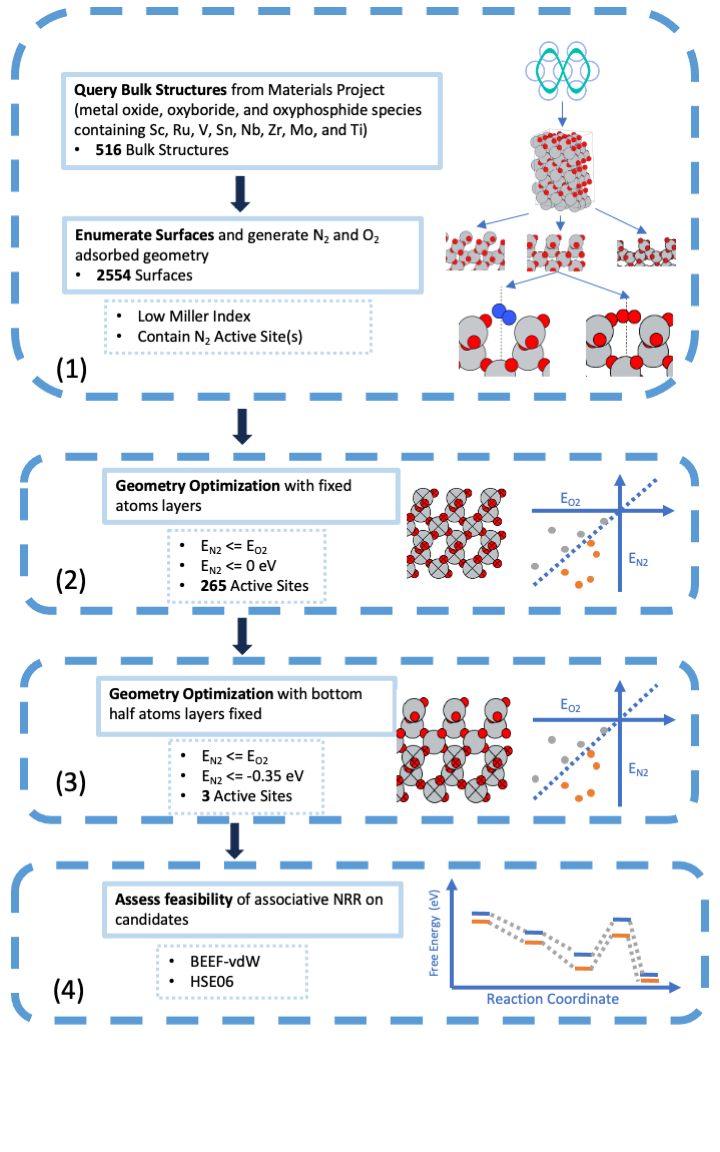
\includegraphics[width=8.6cm]{figures/metal_oxide_figures/Figure 1.png}
\caption{The strategy for screening NRR catalysts. (1) Bulk structures are queried from Materials Project and low Miller index surfaces are generated. N$_2$ active sites are enumerated on each surface. (2) Geometry optimizations are performed with all slab atoms fixed in positions. (3) Geometry optimizations are performed with the bottom half of the slab atoms fixed in positions. (4) NRR free energies are calculated with BEEF-vdW and HSE06 functionals.}
\label{fig:screening_workflow}
\end{center}
\end{figure}

The strategy for the materials screening is illustrated in \ref{fig:screening_workflow}. We used the Materials Project \cite{Jain2013} online database to obtain a pool of bulk metal oxide structures. For this study, we chose transition metal oxide, oxyboride, and oxyphosphide species containing Sc, Ru, V, Sn, Nb, Zr, Mo, and Ti (nonmagnetic metals that are commonly active for nitrogen chemistry in heterogeneous and homogeneous catalysis \cite{ Schrauzer_1977, Schrauzer_2011, schrauzer1986homogeneous, ling2018single, Yandulov_2003, kuriyama2014catalytic, fajardo2017catalytic, Foster2018CatalystsAmmonia, yang2018mechanistic, li2019amorphous, ren2020density, tan2021zr}). We included borides and phosphides due to the fact that boron is known to interact strongly with nitrogen \cite{Jepsen2014BoronnitrogenStorage, Legare2018NitrogenBoron}, and phosphorus is a nutrient that is commonly used in fertilizers and thus phosphides may have practical advantages for fertilizer production. The targeted band gap of the material was set at 0.1 eV to 5.0 eV to identify materials that may be effective photocatalysts. The range was intentionally chosen to be very wide due to well-known errors of GGA functionals in estimating band gaps. There were 516 bulk structures from Materials Project with unique space groups that met these conditions at the time queried, and a full list of bulk structures is given in the SI. From the pool of bulk structures, we generated surfaces from the low Miller index facets of each bulk structure using the \texttt{generate\_all\_slabs} function of \texttt{pymatgen} with a max index of 1 \cite{Ong2013PythonAnalysis}. This results in 2554 low-index surfaces. Then we searched for top, bridge and hollow active sites for N$_2$ binding on these surfaces by applying methods from Materials Project. The O$_2$ adsorbed geometries were obtained by substituting N atoms with O from the preliminary N$_2$ adsorbed geometries. This resulted in 905 active sites that eventually reached SCF convergence in the initial geometry optimization for both N$_2$ and O$_2$. 

The binding energy of an adsorbate on a surface, $E_{ads}$, is calculated according to Equation \ref{eq:binding},
\begin{equation}
    \label{eq:binding}
    E_{ads} = E_{ads+slab}- E_{slab} - E_{gas}
\end{equation}
where $E_{ads+slab}$ is the DFT energy of the adsorbed surface. The reference energies for each system, $E_{slab}$ and $ E_{gas}$, are the DFT energies of the surface slab and adsorbate, respectively. The value of E$_{gas}$ for each adsorbate was calculated as a linear combination of N$_2$, O$_2$, and H$_2$. 

% low fidelity calculations in initial screening
During the initial screening, we performed low-fidelity calculations on all candidate surfaces. For each candidate, all slab layers were fixed in initial positions to reduce computational cost, and geometry optimizations were performed with standard DFT settings to allow the N$_2$ and O$_2$ adsorbate to relax on each surface. The binding energies of both adsorbates on the surface were obtained. We expect that the adsorption energies from this approach will generally overestimate the adsorption strength, since the surface atoms are in a more reactive nonrelaxed state. Thus, only materials that exhibit more stable N$_2$ binding energies than O$_2$ were selected to enter the second round of screening.


In the second round of screening, we performed high-fidelity calculations guided by results from the initial screening. For each adsorption site identified as promising from the initial screening, the top half of the surface layers were unconstrained and additional vacuum space of 6 \textup{~\AA} was added between each layer. Then, geometry optimization was performed via DFT to obtain the lowest N$_2$ and O$_2$ adsorption energies. Similarly to the initial screening, surfaces that exhibit more selective adsorption toward N$_2$ than O$_2$  remain in the candidate materials pool. Then, each candidate surface was visualized and examined carefully. Any surfaces with major reconstruction, adsorbate dissociation, or desorption were re-optimized with additional constraints (e.g. to prevent bond dissociation) or removed from the screening pool if no stable configurations exhibiting stronger N$_2$ than O$_2$ binding could be identified.

In the third round of screening, only three surfaces remained, two of which were based on TiO$_2$ bulk structures. Given the compositional similarity, we selected a single TiO$_2$ structure (with the strongest N$_2$ selectivity) and the VBO$_4$ structure for a final detailed study. We evaluated the feasibility of NRR on the surface by calculating the energetics of each intermediate adsorbed state involved in the NRR reaction at both GGA and hybrid levels of theory.

Every NRR intermediate adsorbate from the associative NRR mechanism \cite{Comer_sustainable} was placed on the surface constructed from the bulk geometry and corresponding Miller indices.
Geometry optimization was performed on each intermediate state using the BEEF-vdW functional, also yielding the corresponding binding energies. Vibrational frequencies and free energies are also computed using the BEEF-vdW functional. Single-point hybrid functional calculations using the HSE06 functional were performed on lowest energy intermediate state as described in Section \ref{sec:DFT}.

All structures from each level of screening, along with scripts used for analysis and DFT simulations, are provided in the Supplementary Information (SI).
The SI containing additional data, code, and materials associated with this study can be found via Zenodo: \url{https://dx.doi.org/10.5281/zenodo.8102485}. The repository includes all screening data, and instruction for querying bulk structures and generating surfaces for the screening.


\section*{Results and Discussion}
\subsection{Material Screening Results}
% Initial screening results: parity plot to compare selectivity; cpu hours

\begin{figure}[h]
\centering
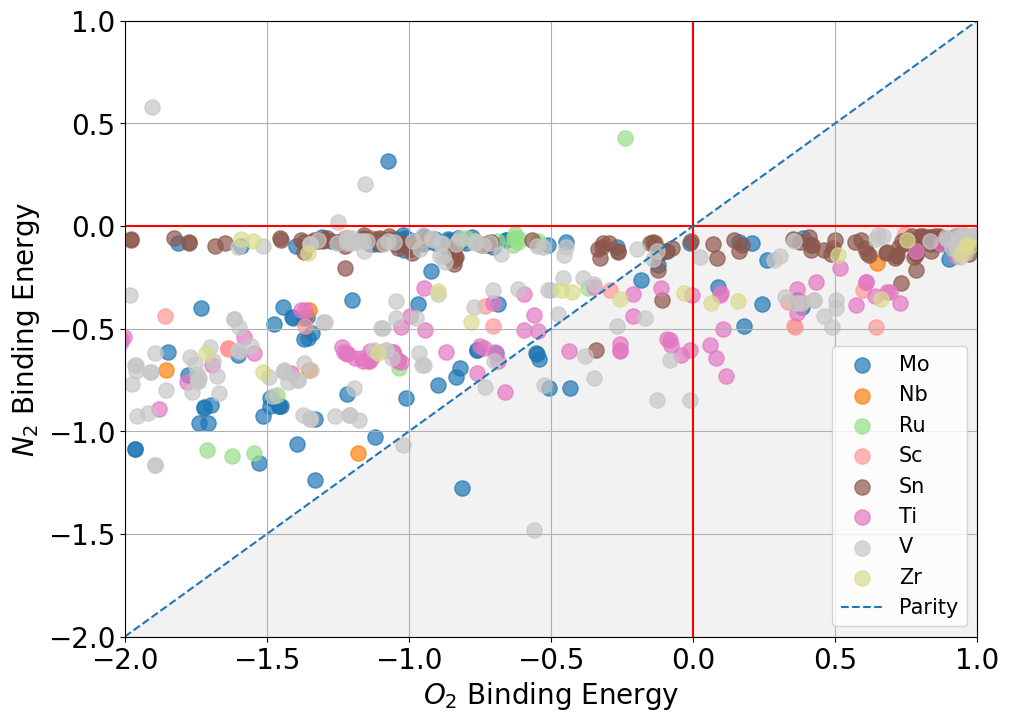
\includegraphics[width=8.6cm]{figures/metal_oxide_figures/Figure 2.png}
\caption{Parity plot of candidate surfaces' N$_2$ vs O$_2$ DFT binding energies. Scatter points \textbf{below} the parity line indicate more favorable N$_2$ binding. The shaded area indicates the desired range of relative binding energies, where $E_{N_2} \le E_{O_2}$.}
% ($E_{N_2}$ $\le$ $E_{O_2}$)
\label{fig:exp_All_binding_comparison}
\end{figure}

\begin{figure}[h]
\centering
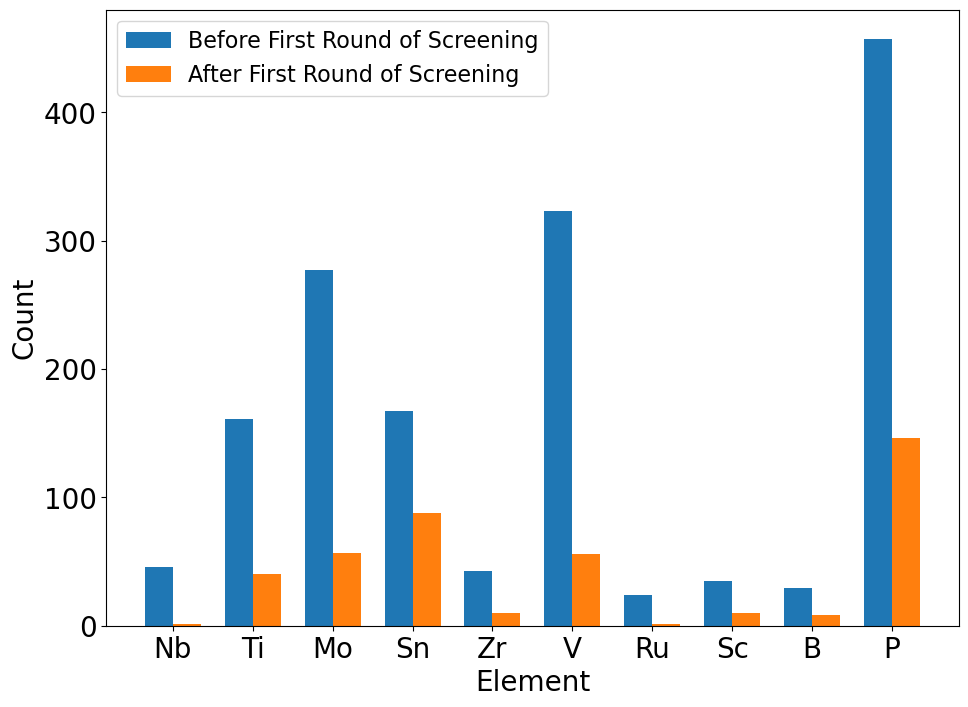
\includegraphics[width=8.6cm]{figures/metal_oxide_figures/Figure 3.png}
\caption{Number of metal oxide candidate species per element. Blue bars indicate the number of total candidates before the first round of screening, and orange bars indicate the number of qualified candidates after the first round of  screening. }
\label{fig:grouped_metal_count_bar_plot}
\end{figure}

A comparison of N$_2$ and O$_2$ obtained for initial screening by low-fidelity calculations is shown in the parity plot in \ref{fig:exp_All_binding_comparison}.  In this initial screening, there are 6606 surface relaxations in total (total compute time of $\sim$500K CPU-hr), including bare and adsorbed surfaces and systems that were ultimately deemed unphysical. In this parity plot, the shaded area indicates the desired range of relative binding. Candidates within this region exhibit more favorable binding towards N$_2$ ($E_{N_2} \le E_{O_2}$). These are candidate surfaces that would enter the second round of screening. These candidate metal compounds include metal species V, Mo, Sn, Zr, Sc, and Ti, and a full list is provided in the SI. The bar plot in \ref{fig:grouped_metal_count_bar_plot} shows a comparison of the abundance of various elements before and after the first round of screening. The results indicate that there is a significant imbalance in the metal types present before and after the screening, and no strong correlation between the proportion of a given metal before and after the screening. This indicates that the screening process is identifying chemical interactions that are distinct to different metal types, rather than simply down-selecting regardless of the metals present. The bar graph also reveals that there are far more oxyphosphides than oxyborides, and despite a large number of oxyborides and oxyphosphides in the initial screening, relatively few exhibited strong N$_2$ adsorption. Naturally, these findings will be influenced by the compositions and types of materials selected, particularly if other classes of materials such as more diverse p-block compounds or metal-organic frameworks were studied.

In the second round of screening, we performed high-fidelity geometry optimizations by allowing the top half of the slab to relax from initial positions. A total of 265 candidate adsorption sites passed the first screening round with stronger reactivity towards N$_2$ than O$_2$. A total of 804 DFT geometry optimizations were performed ($\sim$80K CPU-hr) on these candidate sites. The relative binding energies after the second screening round are shown in \ref{fig:high_fidelity_screening_-0.3}. In many cases, significant surface reconstruction was observed during relaxation. In other cases, the surface N$_2$ desorbed from the active site, resulting in unstable adsorption energies. These findings are consistent with chemical intuition, since the constraints on the slab led to highly reactive surface atoms that are more prone to react with N$_2$, but after relaxation these surface atoms reorganize to bind with each other in the (sub)surface, making them less reactive. The criteria for the second round of screening are $E_{N_2}$ $\le$ $E_{O_2}$, $E_{N_2}$ $\le$ -0.35 eV and $E_{O_2}$ $\le$ 0 eV. The first criterion requires N$_2$ to be adsorbed onto the active site via chemisorption, with a binding energy ($E{N_2}$) of equal to or less than -0.35 eV. This threshold indicates a strong interaction between N$_2$ and the catalyst surface. We also implemented a criterion that ensures that the energy of O$_2$ adsorption ($E{O_2}$) is less than or equal to 0 eV, since positive \ce{O2} adsorption energies are due to computational artifacts (e.g. a less stable spin state in the adsorbed O$_2$ calculation). None of the surfaces that were omitted due to this criterion exhibited strong \ce{N2} adsorption, so a more detailed analysis of these structures was not carried out.

\ref{fig:binding_eng_difference} shows a comparison of N$_2$ and O$_2$ binding energies between the first and second rounds of screening. The parity line represents equal binding energies for the first and second rounds of screening. Approximately 44\% O$_2$ binding energies lie below the parity line, indicating that a considerable portion of candidate active sites exhibit stronger O$_2$ adsorption when the top layers of atoms are allowed to relax. On the other hand, a weaker adsorption strength towards N$_2$ was observed in 84\% of the candidate active sites after the top layers were relaxed. This is likely due to the fact that many of the screened materials are oxides, so it is more likely that the surface reconstructions accommodate the chemisorption of O$_2$. The findings indicate that the screening strategy is unlikely to yield false negatives, since N$_2$ adsorption almost always becomes weaker, but that the lack of surface reconstruction in the first round leads to a large number of false positives.

After the second round of screening, the majority of candidates were deemed unsuitable as they did not exhibit strong and selective N$_2$ adsorption over O$_2$ adsorption. However, we identified three active sites that demonstrated the desired range of relative binding energies, as illustrated in \ref{fig:high_fidelity_screening_-0.3}. 
One oxyboride, VO$_4$B, passed the screening, but all other oxyborides and oxyphosphides were eliminated from consideration. The VO$_4$B surface displays the strongest N$_2$ adsorption (-0.85 eV), but the O$_2$ adsorption is nearly equal (-0.80 eV) in this screening round. 
A total of 29 oxyborides and 457 oxyphosphides were evaluated in the initial screening, with all oxyphosphides eliminated and one oxyboride identified. In comparison, 425 oxides were included in the initial screening round and two promising active sites were identified. Given the small numbers involved, it is difficult to draw strong conclusions about trends between these classes of materials, but the results suggest that oxyborides may be a promising class of materials for further study. Interestingly, all oxide surfaces that passed the second screening round have a bulk stoichiometry of TiO$_2$, although with differing bulk polymorphs and surface facets. Furthermore, the TiO$_2$ R3m (111) active site did not pass the second round screening criteria, but also showed strong and comparable N$_2$ (-0.47 eV) and O$_2$ (-0.50 eV) adsorption strengths. The fact that the three oxide surfaces with the strongest adsorption and selectivity towards N$_2$ all have TiO$_2$ stoichiometry suggests that there may be underlying electronic structure factors that favor interaction between N$_2$ and TiO$_2$, but a more detailed analysis is beyond the scope of this work.


The VBO$_4$ material identified has a modest band gap of 2.07 eV and is metastable with a formation energy 0.089 eV/atom above the hull according to Materials Project \cite{VBO4}, suggesting that this material is an interesting candidate for photocatalytic nitrogen conversion and suitable for a more detailed analysis. Instead of studying all TiO$_2$ sites in more depth, we selected the trigonal titanium oxide (001) active site that exhibits the strongest and most favorable adsorption of N$_2$ (-0.7 eV) over O$_2$ (-0.45 eV). The surface is based on the P3$_1$21 space group of TiO$_2$, a material with a formation energy of 0.049 eV/atom above the most stable polymorph of TiO$_2$ and with a band gap of 3.421 eV according to Materials Project. Given the metastable nature of the material, and the band gap that is similar to rutile and anatase titania, we conclude that it is also suitable for a more detailed study. The fact that only a few active sites pass the second round of screening reflects the difficult nature of identifying oxides that adsorb N$_2$ more selectively than O$_2$, suggesting that this is a ``needle in a haystack'' problem since only 3 out of 905 total active sites screened passed the second round of screening. 

Given the comparison of binding energies between the first and second screening rounds, the substantial computational power needed for each round despite the numerous simplifications, and the rarity of successfully identifying candidate materials, this material screening scheme using fixed geometry calculations is likely impractical for the discovery of additional materials and active sites. Although computing time can be saved when all atoms are fixed, this approach neglects the overly reactive nature of some candidate surfaces, suggesting that geometry optimization is an important part of the screening pipeline. On the other hand, full geometry optimizations of all surfaces using DFT is even more computationally impractical. This suggests that novel screening approaches based on machine learning or fast physics-based models will likely be required to identify additional active sites with strong and selective N$_2$ adsorption. However, as shown in the subsequent section, the surfaces that were identified indeed exhibit strong adsorption of other intermediates and reasonable thermodynamic barriers for nitrogen reduction, suggesting that N$_2$ vs. O$_2$ selectivity is an effective descriptor for identifying surfaces that are promising for nitrogen reduction. Expanding the materials search space to include more hypothetical oxyborides, mixed metal oxides, or additional classes of materials that are known to selectively adsorb N$_2$, such as metal-organic frameworks \cite{Han2023MetalOrganicAmmonia, Khalil2021TheFeatures, Han2023REVIEWReduction}, may also be a promising strategy for future investigations.

\begin{figure}[h]
\centering
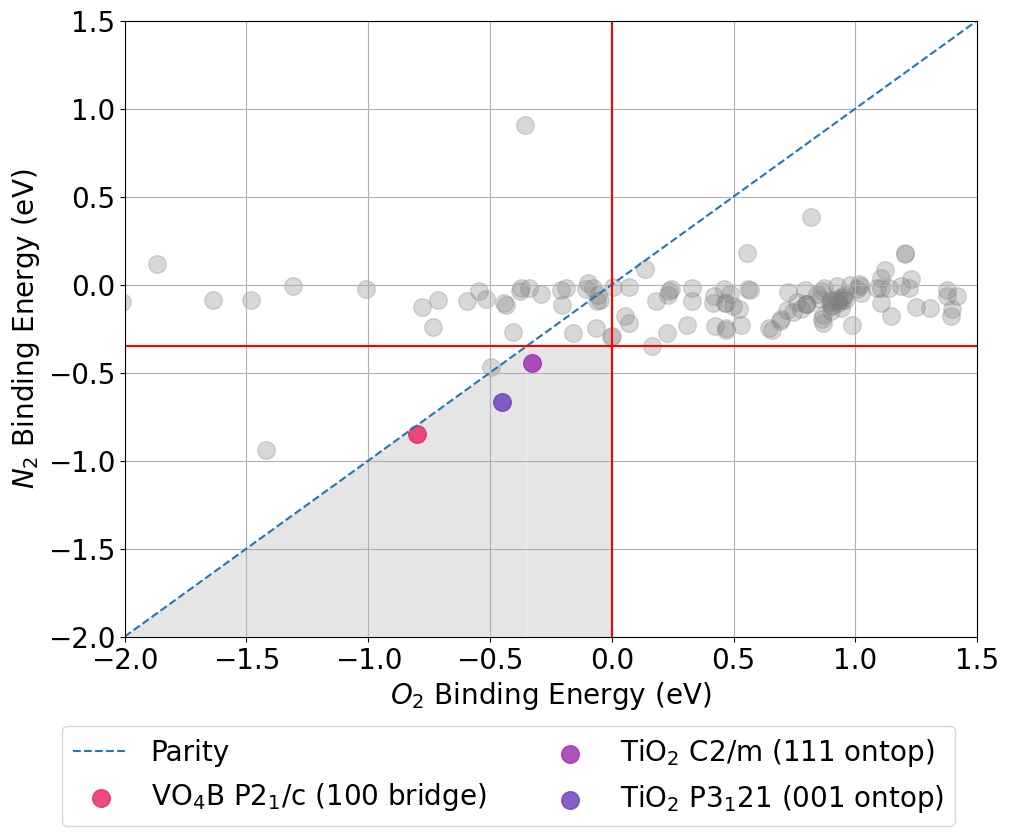
\includegraphics[width=8.6cm]{figures/metal_oxide_figures/Figure 4.png}

\caption{Parity plot of candidate surfaces' N$_2$ vs O$_2$ binding energies from the second round screening. Materials that are deemed promising after the second round screening are colored, others are grey. The shaded area indicates the desired range of relative binding energies, where $E_{N_2}$ $\le$ $E_{O_2}$, $E_{N_2}$ $\le$ -0.35 eV and $E_{O_2}$ $\le$ 0 eV. }
\label{fig:high_fidelity_screening_-0.3}
\end{figure}

\begin{figure}[h]
\centering
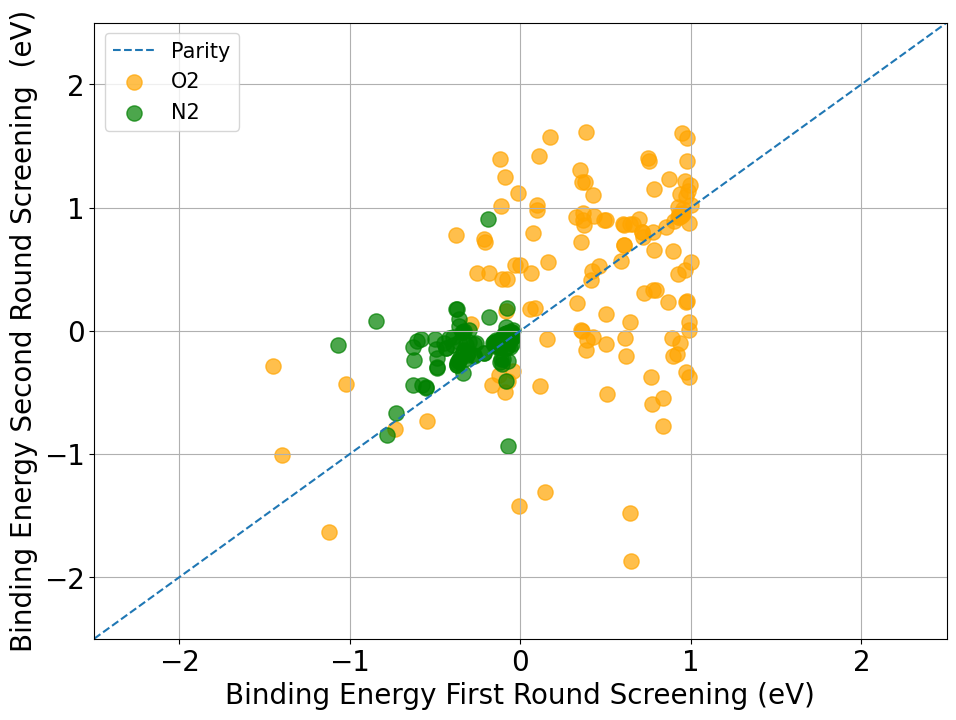
\includegraphics[width=8.6cm]{figures/metal_oxide_figures/Figure 5.png}
\caption{Parity plot of candidate surfaces' N$_2$ vs O$_2$ binding energies, before and after the second round screening.}
\label{fig:binding_eng_difference}
\end{figure}


\begin{figure*}
    \centering
    \begin{subfigure}{0.31\columnwidth}
        \centering
        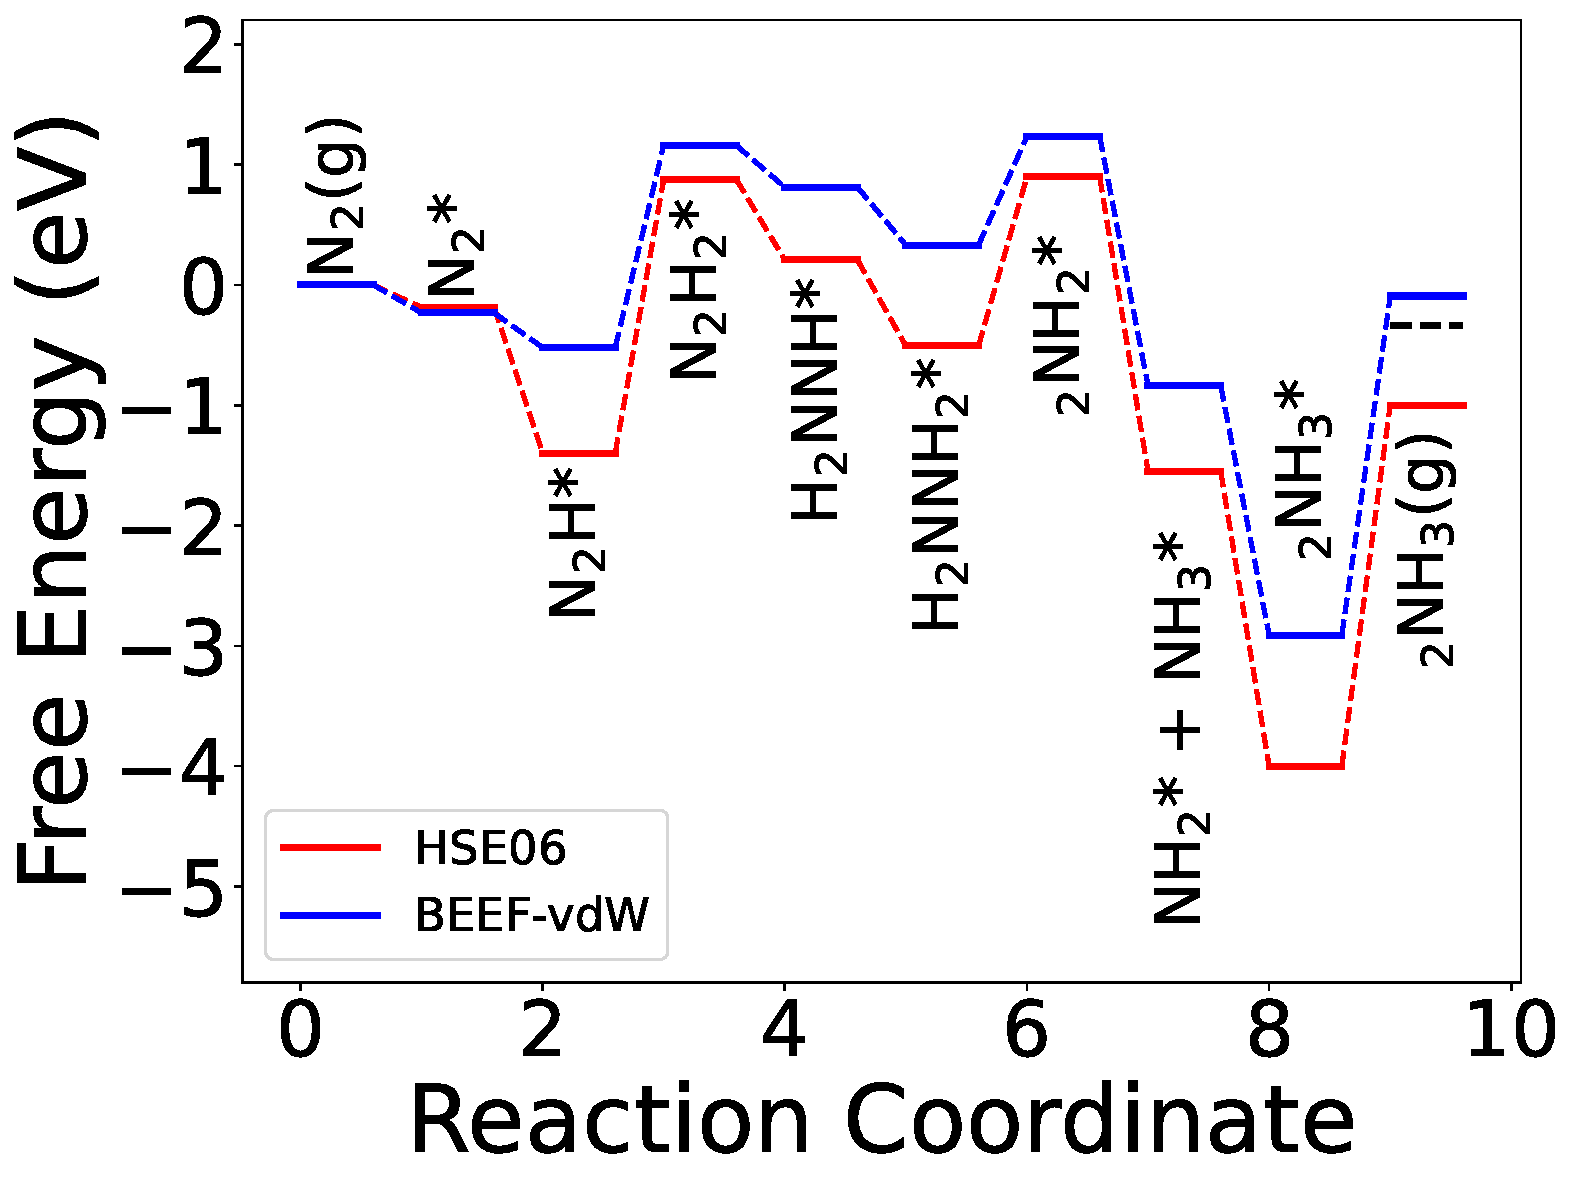
\includegraphics[width=\columnwidth]{figures/metal_oxide_figures/Figure 6a.pdf}
        \caption{}
        \label{fig:FED}
    \end{subfigure}
    % \hfill 
    \begin{subfigure}{0.31\columnwidth}
        \centering
        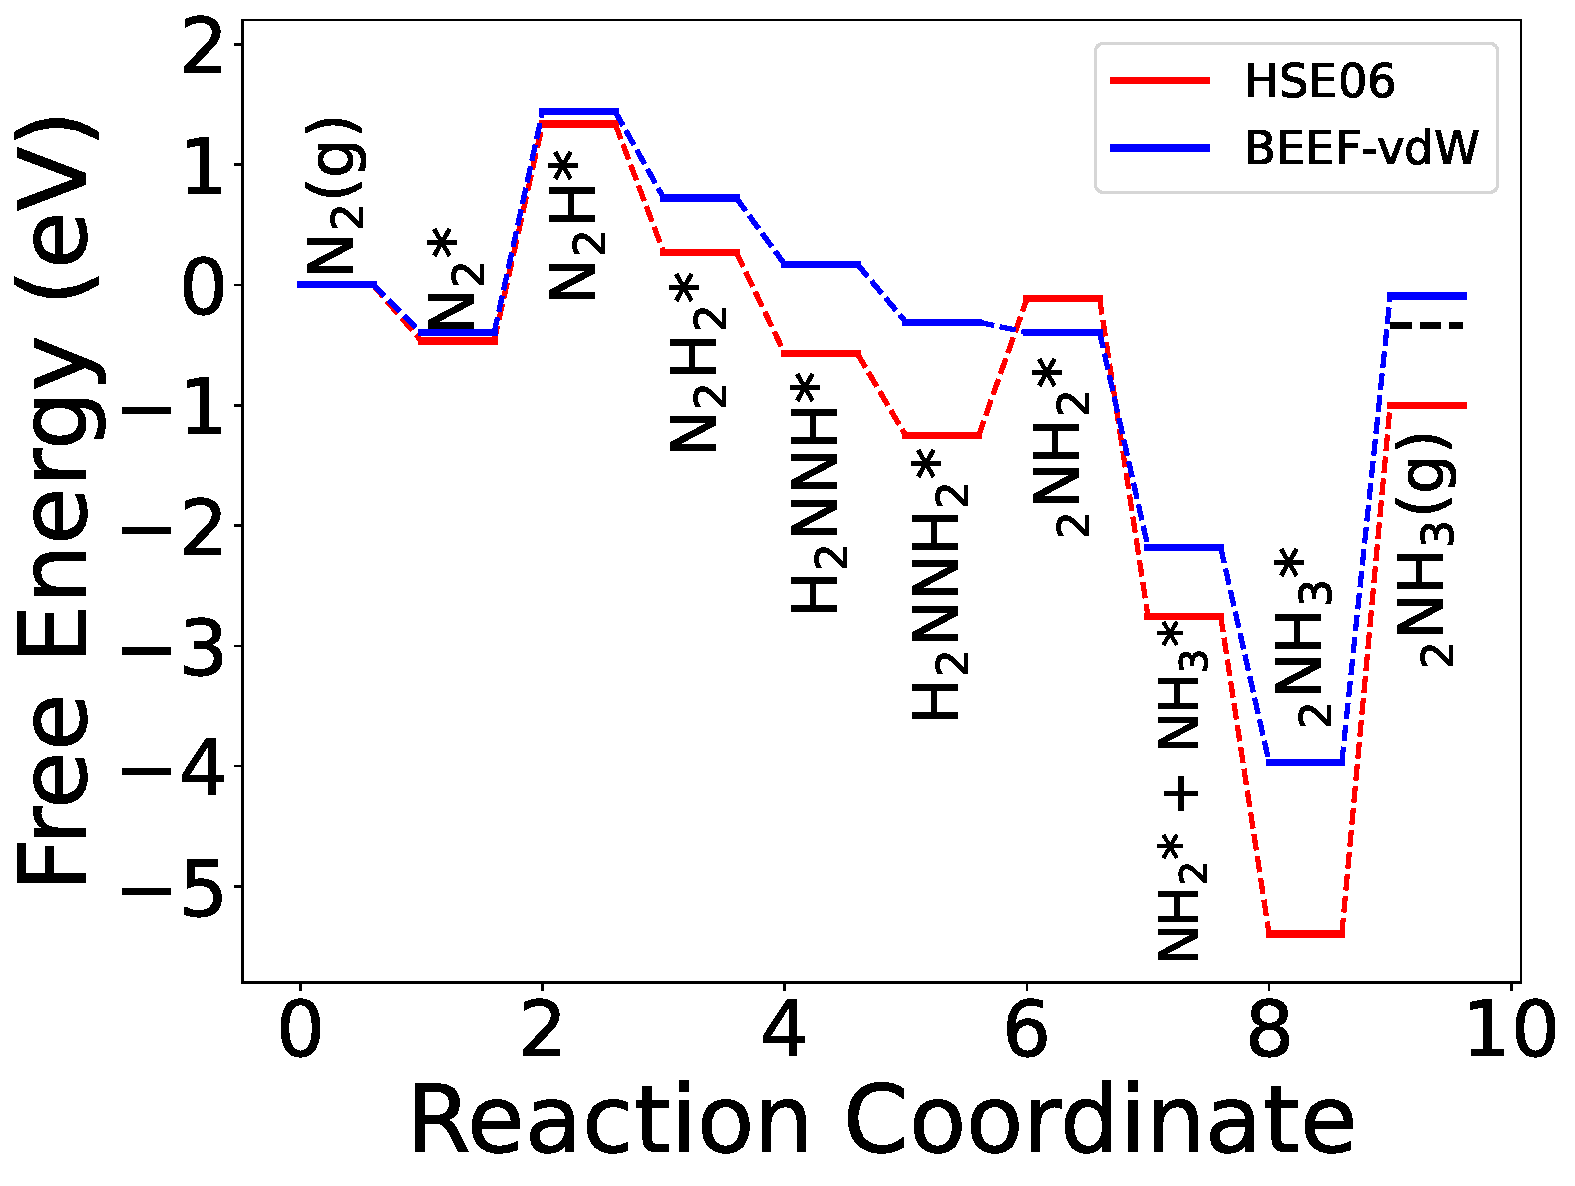
\includegraphics[width=\columnwidth]{figures/metal_oxide_figures/Figure 6b.pdf}
        \caption{}
        \label{fig:VBO_4_FED}
    \end{subfigure}
    % \hfill
    \begin{subfigure}{0.31\columnwidth}
        \centering
        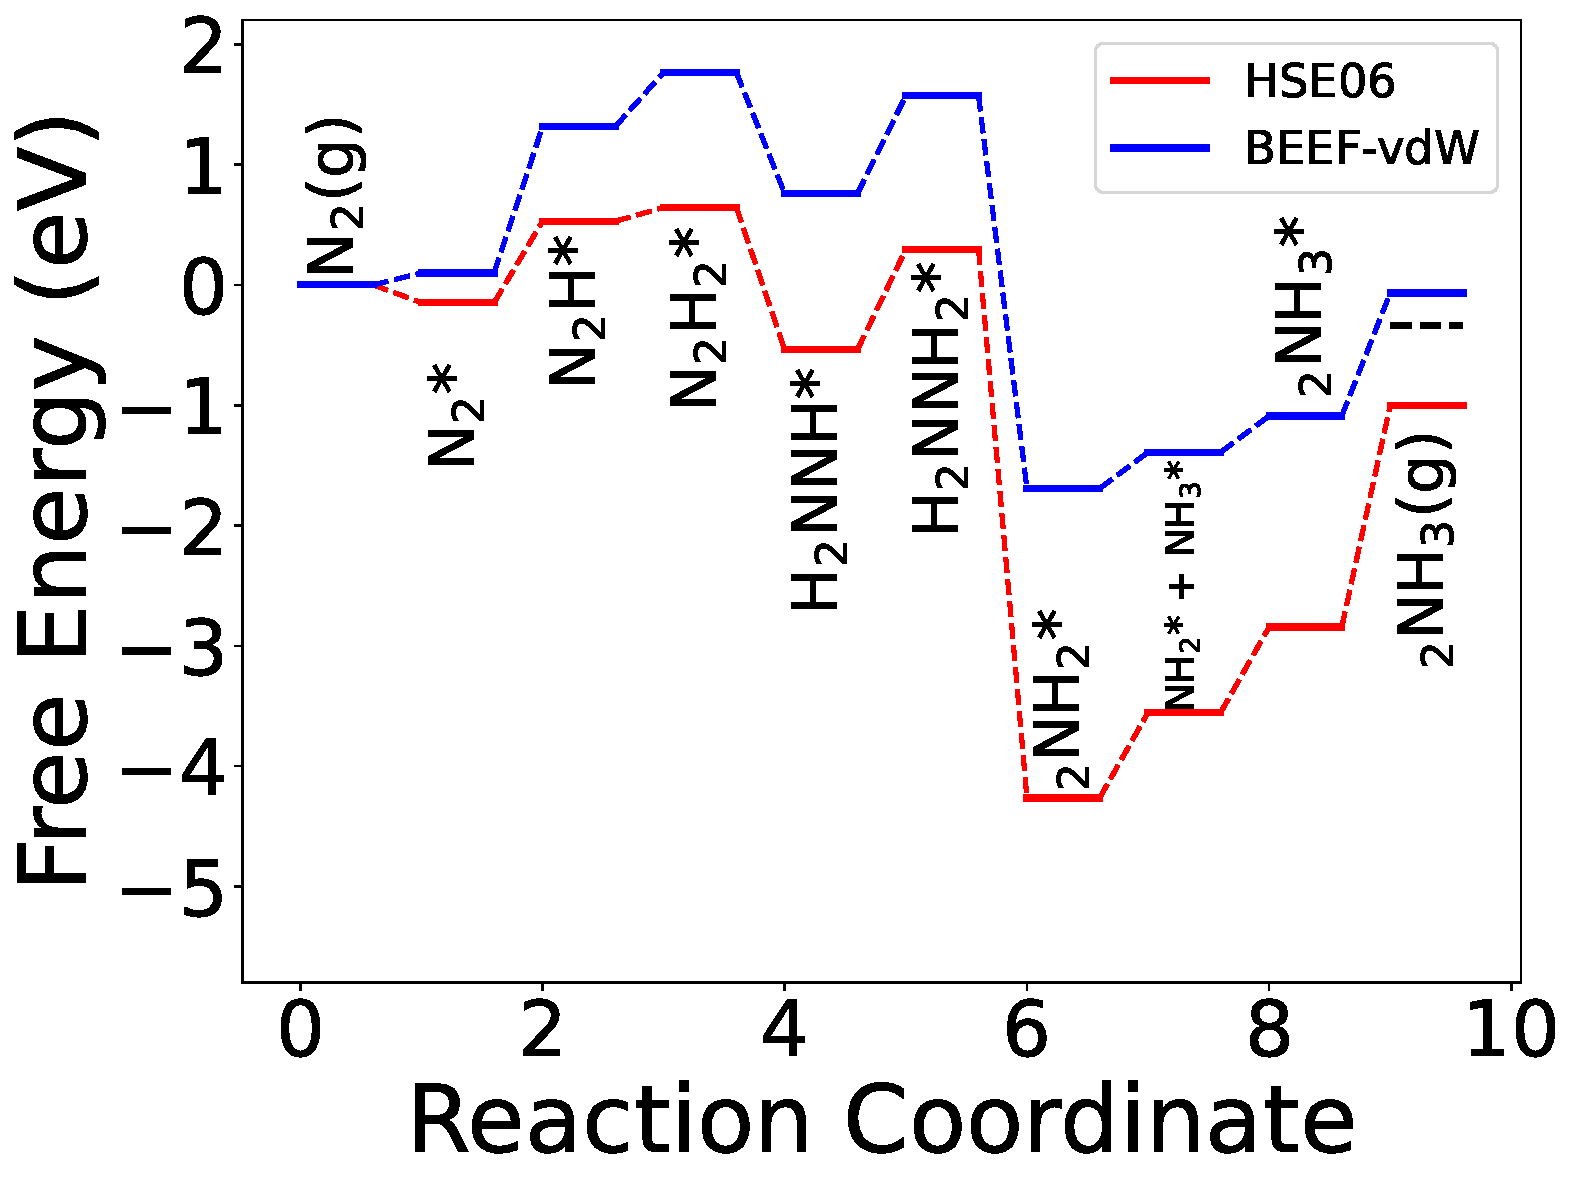
\includegraphics[width=\columnwidth]{figures/metal_oxide_figures/Figure 6c.pdf}
        \caption{}
        \label{fig:ACS_FED}
    \end{subfigure}
    \caption{Free energy diagrams for the associative NRR pathway on the trigonal TiO$_2$ (001) active site (a), the VBO$_4$ (100) active site (b), and the O-br vacancy site of rutile TiO$_2$ (110) (c), both calculated using the BEEF-vdW and HSE06 functionals.}
    \label{fig:combined_FED}
\end{figure*}

\subsection{Nitrogen Reduction Pathway on VBO$_4$ (100) and Trigonal TiO$_2$ (001)}
In the third round of screening, we begin by confirming the selective adsorption of N$_2$ at the HSE06 level of theory for both VBO$_4$ (100) and trigonal TiO$_2$ (001), since HSE06 is known to be more accurate for the treatment of gas phase O$_2$. The findings are confirmed for both surfaces, with VBO$_4$ (100) having an N$_2$ adsorption free energy of -0.82 eV and O$_2$ adsorption energy of -0.40 eV, and trigonal TiO$_2$ (001) having N$_2$ and O$_2$ adsorption energies of -0.62 eV and -0.36 eV respectively.We also briefly consider the possiblity of hydrogen adsorption and evolution, which is known to inhibit electrocatalytic NRR on metals \cite{Singh_2017}. For both surfaces, H* adsorption at the site of N$_2$ adsorption is strongly endergonic (2.24 eV for trigonal TiO$_2$, 0.84 eV for VBO$_4$ with BEEF-vdW), suggesting that it will not directly inhibit N$_2$ adsorption. The free energy diagrams for hydrogen evolution based on adsorption at the most favorable active sites were also calculated, revealing that H* prefers to adsorb to surface oxygen atoms (free energy diagrams and configurations are given in the SI). A full analysis of mixed coverage effects between H* and N$_2$ or O$_2$ is beyond the scope of this work, but these initial results suggest that hydrogen evolution is unlikely to compete with N$_2$ adsorption on either surface.

Next, we compute adsorption energies for all intermediate states in the associative NRR pathway, i.e. $N_xH_y*$ at both the GGA (BEEF-vdW) and hybrid (HSE06) levels of theory as discussed in the methods section. The free energy diagrams can be seen in \ref{fig:FED}, along with the free energy pathway of the associative mechanism on the proposed oxygen vacancy active site of (110) rutile TiO$_2$ for reference \cite{Comer_sustainable}. The trends in adsorption energies between the two functionals are largely consistent, although HSE06 predicts generally stronger adsorption for all species and surfaces, and a much stronger adsorption of N$_2$H for trigonal TiO$_2$. Furthermore, HSE06 significantly overestimates the total reaction energy for NH$_3$ formation, while BEEF-vdW underestimates it by a smaller margin. This indicates that although HSE06 includes Fock exchange and is expected to improve the treatment of the electronic structure of VBO$_4$ and TiO$_2$, the computed adsorption energies are not necessarily more accurate than BEEF-vdW since the bonding between nitrogen and hydrogen in the gas phase has significant errors. A detailed comparison of the level of theory is beyond the scope of this work, but the fact that both follow a similar trend provides strong evidence that the qualitative conclusions are reliable.

The free energy diagram for VBO$_4$ is generally similar to that of the oxygen vacancy on rutile (110), with a significant thermodynamic barrier for N$_2$H formation, followed by mostly exergonic steps to form strongly bound NH$_3$. One difference is the dissociation of N$_2$H$_4$, which is exergonic with BEEF-vdW but endergonic by 1.1 eV with HSE06. The N$_2$H$_2$ intermediate is more stable on VBO$_4$ than on rutile, and the height of the thermodynamic barrier of $\sim$1.4 eV between gas-phase N$_2$ and N$_2$H is slightly lower or higher than the barrier on rutile (110), depending on the level of theory. The thermodynamic barrier for N$_2$H formation is significantly higher than the $\sim$0.75 eV threshold for processes that are active at room temperature \cite{Iriawan_2021}, but the selective adsorption of N$_2$ and strong interaction with other intermediates suggest that other mechanisms that stabilize or avoid N$_2$ H may allow ammonia production on this surface. A full exploration of possible mechanisms is beyond the scope of this work, so we tentatively conclude that although the VBO$_4$ surface exhibits strong N$_2$ activity, it is not expected to be active for ammonia synthesis.

The free energy diagram for trigonal TiO$_2$ (001) exhibits significant thermodynamic barriers for the conversion of N$_2$H to N$_2$H$_2$ (1.7 or 2.3 eV with BEEF-vdW or HSE06), and for the dissociation of N$_2$H$_4$ to form NH$_2$ (0.9 or 1.4 eV with BEEF-vdW or HSE06). The high thermodynamic barrier for N$_2$H hydrogenation on the trigonal TiO$_2$ (001) active site is due to very stable adsorption of the *N$_2$H intermediate state, which is in contrast to the VBO$_4$ and rutile (110) surfaces, where formation of N$_2$H is one of the most endergonic steps. Indeed, N$_2$H formation has been identified as the likely rate-limiting step for numerous NRR catalysts in the literature \cite{Skulason_2012, Ji2023UnifyingSurfaces,Bourgeois1988AAmmonia}, indicating that the trigonal TiO$_2$ (001) exhibits notable stabilization of N$_2$H. The fact that N$_2$H formation is exergonic compared to the initial state suggests that under reaction conditions the N$_2$H coverage will likely increase, effectively increasing the free energy of the state due to configurational entropy and thus lowering the barrier for N$_2$H formation and providing a possible route for experimental validation via spectroscopic studies. In the limit that adsorbed N$_2$H is in equilibrium with the initial state (causing the free energies to be identical by definition) the barrier to N$_2$H$_2$ formation would decrease to $\sim$1 eV, bringing it close to the $\sim$0.75 eV limit needed for an active NRR catalyst \cite{Iriawan_2021}. 

The barrier that arises due to strong NH$_3$ adsorption exists to varying degrees for most surfaces, although NH$_3$ adsorption is stronger on the trigonal TiO$_2$ (001) surface than the VBO$_4$ or rutile (110) surfaces. This barrier is less important for NRR, since the free energy of gas or solution phase NH$_3$ will decrease at low concentrations. In the absence of significant desorption barriers, ammonia produced will equilibrate with the final state, effectively lowering this thermochemical barrier but limiting the conversion that is possible. In general, analysis of the free energy pathway suggests that the active site of trigonal TiO$_2$ has comparable or lower thermochemical barriers to the oxygen vacancy of rutile (110) for the conversion of N$_2$ to adsorbed NH$_3$, although more detailed investigations are needed to establish the most appropriate exchange correlation functional, explore alternative pathways such as carbon-assisted N$_2$ fixation \cite{Comer2018TheTitania}, and identify kinetic barriers. Furthermore, it is possible that the trigonal TiO$_2$ (001) site exists in polycrystalline TiO$_2$ and works synergistically with other sites by stabilizing N$_2$H.

\begin{figure}[h]
\centering
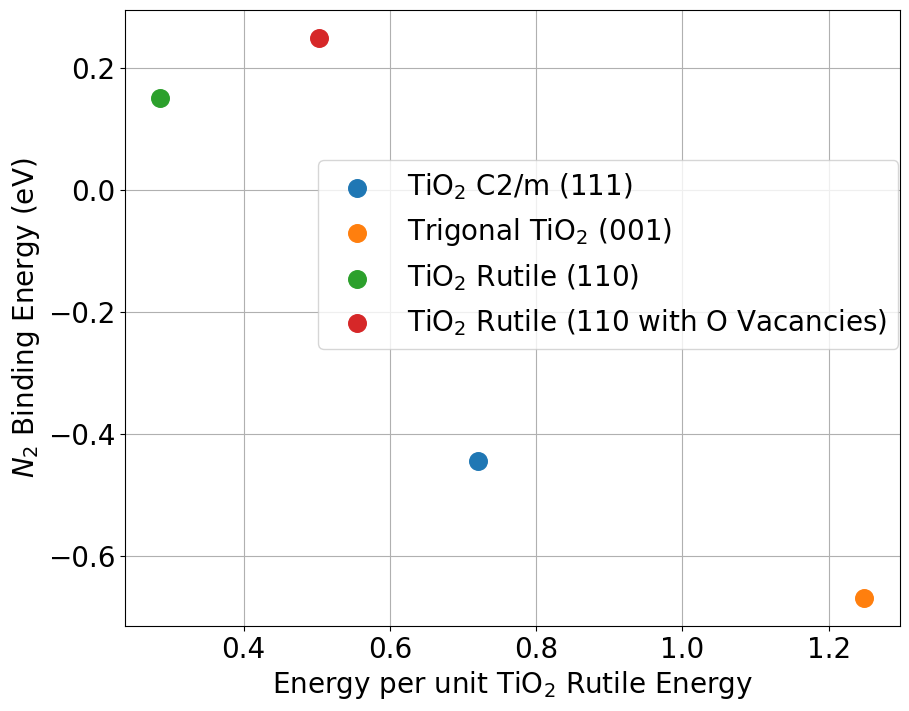
\includegraphics[width=8.6cm]{figures/metal_oxide_figures/Figure 7.png}
\caption{Surface formation energy of various candidate promising active sites vs the adsorption energy of N$_2$ evaluated, relative to pristine rutile (110) and rutile (110) with O vacancies. }
\label{fig:formation_vs_ads}
\end{figure}

Next, we use HSE06 to conduct a detailed investigation of the band gap and band edge positions of both trigonal TiO$_2$ and VBO$_4$. The results are shown in \ref{fig:bandgap_alignment}, and reveal that the band gap of trigonal TiO$_2$ and VBO$_4$ are 3.42 eV and 3.46 eV respectively. These gaps are too large for highly efficient capture of solar photons, but may enable low-efficiency conversion. Moreover, the band alignment of VBO$_4$ indicates that the edge of the conduction band lies well below the redox potential for N$_2$ reduction to NH$_3$, indicating that this material is probably not suitable for direct photocatalytic N$_2$ fixation, although it may still be interesting as a cocatalyst or as a catalyst for N$_2$ oxidation. On the other hand, the edge of the conduction band of the trigonal TiO$_2$ is 0.85 V above the NH$_3$ redox potential, indicating that there is a stronger driving force for NH$_3$ reduction than for other polymorphs of TiO$_2$ \cite{Comer2018AnalysisTiO2110}.

\begin{figure}[h]
\centering
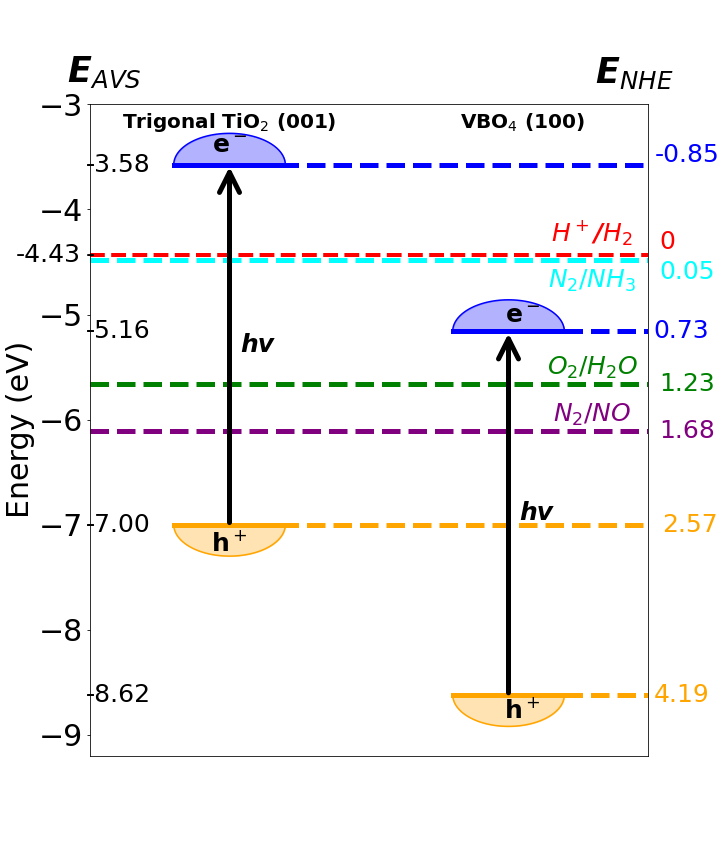
\includegraphics[width=8.6cm]{figures/metal_oxide_figures/Figure 8.png}

\caption{Band edge positions of trigonal TiO$_2$ (001) (left) and VBO$_4$ (100) (right). Both calculated using the BEEF-vdW and HSE06 functionals. E$_{NHE}$ and E$_{AVS}$ denote energy levels relative to a normal hydrogen electrode (NHE) and the absolute vacuum scale (AVS), respectively.
 }
\label{fig:bandgap_alignment}
\end{figure}

 
Given that nearly all the surfaces that were identified from the second round of screening (Fig. 
\ref{fig:high_fidelity_screening_-0.3}) are TiO$_2$, it is relevant to consider the stability of these surfaces to determine how likely they are to occur in polycrystalline TiO$_2$ or how difficult they would be to synthesize. \ref{fig:formation_vs_ads} compares the N$_2$ adsorption and formation energies of all TiO$_2$ surfaces qualified in the second round of screening. The relative surface formation energies, $E_{surf,rel}$, are computed relative to pristine rutile TiO$_2$, one of the most stable forms of titania, as shown in Equation \ref{relative surface formation energy}, where $E_{surf}$ is the total energy of the surface divided by the total number of TiO$_2$ units in the slab and $E_{rutile}$ is the total energy of the bulk rutile per unit TiO$_2$ in the bulk structure.

\begin{equation}
E_{surf, rel} = E_{surf} - E_{rutile}
\label{relative surface formation energy}
\end{equation} 

Although trigonal TiO$_2$ displays the strongest N$_2$ adsorption, and the most selective N$_2$ adsorption over O$_2$, it also displays the highest surface energy. This suggests it may be difficult to synthesize and is unlikely to form spontaneously, but the fact that O$_2$ does not strongly adsorb or spontaneously dissociate suggests that the site will likely be meta-stable if it does form.

The trigonal TiO$_2$ polymorph has not been experimentally reported to our knowledge and has not been specifically tested for photocatalytic nitrogen fixation. 
However, other titania polymorphs and nanoparticles have been reported to photocatalytically produce ammonia in a number of studies \cite{Comer_sustainable, Comer2019ProspectsFertilizers, Hirakawa_2017, Lu1994, Benkoula2015, Rusu2001, Henderson_2011, Cheng2011}, including under aerobic conditions \cite{Liu_2022}. The performance has also been reported to vary significantly depending on the polymorph and even supplier of the catalyst \cite{Hirakawa_2017}, and there are numerous inconsistent results in the literature. The presence or influence of trigonal TiO$_2$ active sites has never been suggested, but the meta-stable nature of the polymorph suggests that it may appear in polycrystalline titania, or that some defect sites may have a similar structure. The presence and role of these non-standard TiO$_2$ polymorphs and surface structures may be relevant for photocatalytic ammonia synthesis, especially under aerobic conditions. In addition, the finding suggests that intentional synthesis of the trigonal polymorph may be a promising strategy to increasing photocatalytic ammonia performance, especially if the abundance of the 001 facet \cite{Roy2013SynergyPhotocatalysis, Kislov2022EffectCompound, YongChae2003PreparationFilms, Liao2013ActivatingFacets, Yu2012Low-costPhotoactivities} can be enhanced through capping agents or other techniques.



\section*{Conclusion}
The high-throughput DFT screening used in this work successfully identified a novel titanium dioxide active site that exhibits selective adsorption of N$_2$ over O$_2$ as well as promising energetics for the NRR reaction, and a VBO$_4$ active site that selectively adsorbs N$_2$ over O$_2$, but exhibits a high thermodynamic barrier for N$_2$H formation. The screening process revealed that surface relaxation and reconstruction can substantially affect reactivity and selectivity toward N$_2$, suggesting that future screening strategies should take reconstruction into account. However, the computational cost of the DFT-only screening process will likely be prohibitive for relaxations, suggesting that machine-learned force fields or other techniques should be explored. However, the findings also reveal that evaluating N$_2$ vs. O$_2$ selectivity is a promising route to substantially reduce the search space and identify active sites that are metastable and exhibit strong reactivity toward N$_2$.

The results of the screening process revealed several interesting active sites with TiO$_2$ and VBO$_4$ stoichiometry. Among them, the VBO$_4$ surface demonstrated the strongest N$_2$ adsorption and the trigonal TiO$_2$ (001) surface exhibited the strongest selectivity towards N$_2$. A detailed investigation of both surfaces at the GGA (BEEF-vdW) and hybrid (HSE06) levels of theory was conducted. The results show that the selective adsorption of N$_2$ over O$_2$ holds at both levels of theory, and that N$_2$H formation is limiting on the VBO$_4$ surface, while the trigonal TiO$_2$ surface exhibits a particularly strong reactivity toward N$_2$H. Free energy diagrams indicate that the trigonal TiO$_2$ surface exhibits a somewhat large thermochemical barriers for conversion of N$_2$H to N$_2$H$_2$ (1.7 or 2.3 eV for BEEF-vdW or HSE06), but these barriers occur due to the strongly exergonic adsorption of N$_2$H, and may become surmountable at high N$_2$H coverages. These findings suggest that trigonal TiO$_2$ may exhibit increased photocatalytic NRR performance, or that defect sites with topologies similar to the active sites of trigonal TiO$_2$ (001) may contribute to photocatalytic ammonia synthesis in polycrystalline titania catalysts, especially under aerobic conditions. The findings also suggest that oxyborides may be a promising material class for future screening studies and that the surfaces of VBO$_4$ and trigonal TiO$_2$ surfaces may also be of interest for other applications, such as air separation. Furthermore, the fundamental chemistry underlying the selective adsorption of inert N$_2$ over reactive O$_2$ on oxide surfaces is not well understood and requires further investigation. In general, the screening process was successful in identifying an interesting trigonal TiO$_2$ active site structure, and revealed that surfaces capable of selectively adsorbing N$_2$ over O$_2$ are relatively rare, at least among the compounds included in this screening process.
